\documentclass{standalone}
\usepackage{graphicx}	
\usepackage{amssymb, amsmath, amsthm}
\usepackage{color}

\usepackage{tikz}
\usetikzlibrary{intersections, backgrounds, arrows}

\definecolor{light}{RGB}{220, 188, 188}
\definecolor{mid}{RGB}{185, 124, 124}
\definecolor{dark}{RGB}{143, 39, 39}
\definecolor{highlight}{RGB}{180, 31, 180}
\definecolor{gray10}{gray}{0.1}
\definecolor{gray20}{gray}{0.2}
\definecolor{gray30}{gray}{0.3}
\definecolor{gray40}{gray}{0.4}
\definecolor{gray60}{gray}{0.6}
\definecolor{gray70}{gray}{0.7}
\definecolor{gray80}{gray}{0.8}
\definecolor{gray90}{gray}{0.9}
\definecolor{gray60}{gray}{0.95}

\tikzset{
  double -latex/.style args={#1 colored by #2 and #3}{    
    -latex,line width=#1,#2,
    postaction={draw,-latex,#3,line width=(#1)/3,shorten <=(#1)/4,shorten >=4.5*(#1)/3},
  },
  double round cap-latex/.style args={#1 colored by #2 and #3}{    
    round cap-latex,line width=#1,#2,
    postaction={draw,round cap-latex,#3,line width=(#1)/3,shorten <=(#1)/4,shorten >=4.5*(#1)/3},
  },
  double round cap-stealth/.style args={#1 colored by #2 and #3}{
    round cap-stealth,line width=#1,#2,
    postaction={round cap-stealth,draw,,#3,line width=(#1)/3,shorten <=(#1)/3,shorten >=2*(#1)/3},
  },
  double -stealth/.style args={#1 colored by #2 and #3}{
    -stealth,line width=#1,#2,
    postaction={-stealth,draw,,#3,line width=(#1)/3,shorten <=(#1)/3,shorten >=2*(#1)/3},
  },
}


\begin{document}

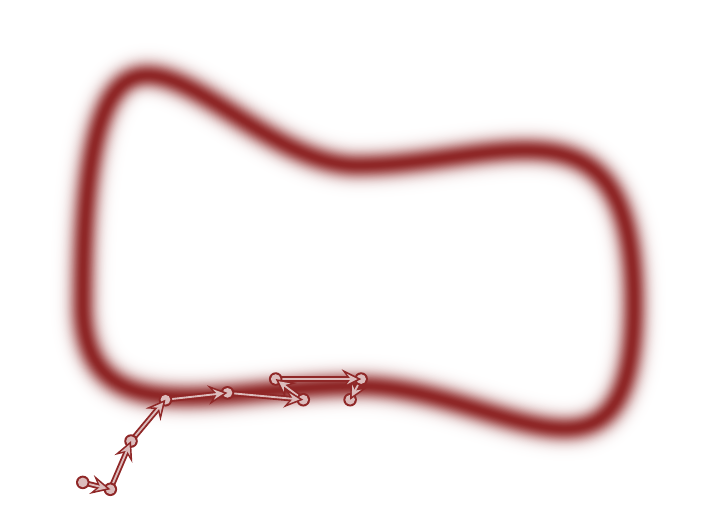
\begin{tikzpicture}[scale=0.35, thick]

  \begin{scope}
  \clip (-12, -7) rectangle (12, 10);
  \foreach \i in {1, 0.99, ..., 0} {
    \pgfmathsetmacro{\prop}{100 * exp(-10.0 * \i * \i)};
    \colorlet{custom}{dark!\prop!white};
    \draw[line width={30 * \i}, color=custom] 
      (-10, 0) .. controls (-10, 15) and (-5, 5) .. (0, 5)
      .. controls (5, 5) and (10, 8) .. (10, 0)
      .. controls (10, -8) and (5, -3) .. (0, -3)
      .. controls (-5, -3) and (-10, -5) .. (-10, 0);
  }

  \fill[color=dark] (-0.3, -3.5) circle (7pt);  
  \fill[color=light] (-0.3, -3.5) circle (5pt);  
    
  \draw[double round cap-stealth=2pt colored by dark and light] (0.1, -2.75) -- (-0.3, -3.5);
  
  \fill[color=dark] (0.1, -2.75) circle (7pt);  
  \fill[color=light] (0.1, -2.75) circle (5pt);
  
  \draw[double round cap-stealth=2pt colored by dark and light] (-3, -2.75) -- (0.1, -2.75);
  
  \fill[color=dark] (-3, -2.75) circle (7pt);  
  \fill[color=light] (-3, -2.75) circle (5pt);

  \draw[double round cap-stealth=2pt colored by dark and light] (-2, -3.5) -- (-3, -2.75);
   
  \fill[color=dark] (-2, -3.5) circle (7pt);  
  \fill[color=light] (-2, -3.5) circle (5pt);
  
  \draw[double round cap-stealth=2pt colored by dark and light] (-4.75, -3.25) -- (-2, -3.5);
   
  \fill[color=dark] (-4.75, -3.25) circle (7pt);  
  \fill[color=light] (-4.75, -3.25) circle (5pt);
  
  \draw[double round cap-stealth=2pt colored by dark and light] (-7, -3.5) -- (-4.75, -3.25);
  
  \fill[color=dark] (-7, -3.5) circle (7pt);  
  \fill[color=light] (-7, -3.5) circle (5pt);
  
  \draw[double round cap-stealth=2pt colored by dark and light] (-8.25, -5) -- (-7, -3.5);
  
  \fill[color=dark] (-8.25, -5) circle (7pt);  
  \fill[color=light] (-8.25, -5) circle (5pt);

  \draw[double round cap-stealth=2pt colored by dark and light] (-9, -6.75) -- (-8.25, -5);

  \fill[color=dark] (-9, -6.75) circle (7pt);  
  \fill[color=light] (-9, -6.75) circle (5pt);
  
  \draw[double round cap-stealth=2pt colored by dark and light] (-10, -6.5) -- (-9, -6.75);
  
  \fill[color=dark] (-10, -6.5) circle (7pt);  
  \fill[color=light] (-10, -6.5) circle (5pt);
  
  
  \end{scope} 
  
\end{tikzpicture}


\end{document}  